%% LyX 2.3.4.2 created this file.  For more info, see http://www.lyx.org/.
%% Do not edit unless you really know what you are doing.
\documentclass[handout,english,dvipsnames,aspectratio=169]{beamer}
\usepackage{mathptmx}
\usepackage{eulervm}
\usepackage[T1]{fontenc}
\usepackage[latin9]{inputenc}
\usepackage{babel}
\usepackage{amstext}
\usepackage{amssymb}
\usepackage{graphicx}
\usepackage{ifthen}
\usepackage{xcolor}
\usepackage{xspace}
\usepackage{tikz}
\usetikzlibrary{tikzmark}
\usetikzlibrary{calc}
\usepackage{pgfplots}
%\pgfplotsset{compat=1.17}
\usepackage{booktabs}



\ifx\hypersetup\undefined
  \AtBeginDocument{%
    \hypersetup{unicode=true,pdfusetitle,
 bookmarks=true,bookmarksnumbered=false,bookmarksopen=false,
 breaklinks=false,pdfborder={0 0 0},pdfborderstyle={},backref=false,colorlinks=true,
 allcolors=NYUPurple,urlcolor=LightPurple}
  }
\else
  \hypersetup{unicode=true,pdfusetitle,
 bookmarks=true,bookmarksnumbered=false,bookmarksopen=false,
 breaklinks=false,pdfborder={0 0 0},pdfborderstyle={},backref=false,colorlinks=true,
 allcolors=NYUPurple,urlcolor=LightPurple}
\fi

\makeatletter

%%%%%%%%%%%%%%%%%%%%%%%%%%%%%% LyX specific LaTeX commands.
%% Because html converters don't know tabularnewline
\providecommand{\tabularnewline}{\\}

%%%%%%%%%%%%%%%%%%%%%%%%%%%%%% Textclass specific LaTeX commands.
% this default might be overridden by plain title style
\newcommand\makebeamertitle{\frame{\maketitle}}%
% (ERT) argument for the TOC
\AtBeginDocument{%
  \let\origtableofcontents=\tableofcontents
  \def\tableofcontents{\@ifnextchar[{\origtableofcontents}{\gobbletableofcontents}}
  \def\gobbletableofcontents#1{\origtableofcontents}
}

%%%%%%%%%%%%%%%%%%%%%%%%%%%%%% User specified LaTeX commands.
\usetheme{CambridgeUS} 
\beamertemplatenavigationsymbolsempty


% Set Color ==============================
\definecolor{NYUPurple}{RGB}{87,6,140}
\definecolor{LightPurple}{RGB}{165,11,255}


\setbeamercolor{title}{fg=NYUPurple}
\setbeamercolor{frametitle}{fg=NYUPurple}

\setbeamercolor{background canvas}{fg=NYUPurple, bg=white}
\setbeamercolor{background}{fg=black, bg=NYUPurple}

\setbeamercolor{palette primary}{fg=black, bg=gray!30!white}
\setbeamercolor{palette secondary}{fg=black, bg=gray!20!white}
\setbeamercolor{palette tertiary}{fg=gray!20!white, bg=NYUPurple}

\setbeamertemplate{headline}{}
\setbeamerfont{itemize/enumerate body}{}
\setbeamerfont{itemize/enumerate subbody}{size=\normalsize}

\setbeamercolor{parttitle}{fg=NYUPurple}
\setbeamercolor{sectiontitle}{fg=NYUPurple}
\setbeamercolor{sectionname}{fg=NYUPurple}
\setbeamercolor{section page}{fg=NYUPurple}
%\setbeamercolor{description item}{fg=NYUPurple}
%\setbeamercolor{block title}{fg=NYUPurple}

\setbeamertemplate{blocks}[rounded][shadow=false]
\setbeamercolor{block body}{bg=normal text.bg!90!NYUPurple}
\setbeamercolor{block title}{bg=NYUPurple!30, fg=NYUPurple}



\AtBeginSection[]{
  \begin{frame}
  \vfill
  \centering
\setbeamercolor{section title}{fg=NYUPurple}
 \begin{beamercolorbox}[sep=8pt,center,shadow=true,rounded=true]{title}
    \usebeamerfont{title}\usebeamercolor[fg]{title}\insertsectionhead\par%
  \end{beamercolorbox}
  \vfill
  \end{frame}
}

\makeatother

\setlength{\parskip}{\medskipamount} 

\input ../macros

\begin{document}
\input ../rosenberg-macros

\title[DS-GA 1003]{Probabilistic Modeling}
\author{Ravid Shwartz Ziv}
\date{Feb 28, 2023}
\institute{CDS, NYU}

\makebeamertitle
\mode<article>{Just in article version}

\begin{frame}{Contents}
\tableofcontents{}
\end{frame}

\begin{frame}{Logistics}
\begin{itemize}
    \item Midterm (also see announcement on Brightspace)
\begin{itemize}
\item Date and time: March 8 5pm--7pm ET 
\item Coverage: up to kernel methods (not including this week)
\item Review: this week's lab
\item Difficulty: easier than last year
\end{itemize}
\end{itemize}
\end{frame}

\section{Overview}
\begin{frame}
{Why probabilistic modeling?}
\begin{itemize}
\item A unified framework that covers many models, \eg linear regression, logistic regression
\item Learning as \textbf{statistical inference}
\item Principled ways to incorporate your belief on the data generating distribution (inductive biases)
\end{itemize}
\end{frame}

\begin{frame}
{Today's lecture}
\begin{itemize}
\item Two ways to model how the data is generated:
\pause
\begin{itemize}
\item \textbf{Conditional}: $p(y\mid x)$
\item \textbf{Generative}: $p(x, y)$
\end{itemize}
\pause
\item How to estimate the parameters of our model? Maximum likelihood estimation.
\pause
\item Compare and contrast conditional and generative models.
\end{itemize}
\end{frame}

\section{Conditional models}
\subsection{Recap: linear regression}

\begin{frame}{Linear regression}
Linear regression is one of the most important methods in machine learning and statistics.

\textbf{Goal}:  Predict a real-valued \textbf{target} $y$ (also called {response})
from a vector of \textbf{features} $x$ (also called {covariates}).
\pause

\textbf{Examples}:
\begin{itemize}
\item Predicting house price given location, condition, build year etc.
\item Predicting medical cost of a person given age, sex, region, BMI etc.
\item Predicting age of a person based on their photos.
\end{itemize}
\end{frame}

\begin{frame}{Problem setup}
\begin{description}
\item[Data] Training examples $\mathcal{D} = \{(x^{(n)}, y^{(n)})\}_{n=1}^N$,
where $x \in \mathbb{R}^d$ and $y \in \mathbb{R}$.
\pause{}

\item[Model] A \emph{linear} function $h$ (parametrized by $\theta$)
to predict $y$ from $x$:
\begin{align}
h(x) = \sum_{i=0}^d \theta_i x_i = \theta^T x,
\end{align}
where $\theta \in \mathbb{R}^d$ are the \textbf{parameters} (also called weights).
\end{description}
\pause{}

Note that
\begin{itemize}
\item We incorporate the \textbf{bias term} (also called the intercept term) into $x$ (i.e. $x_0 = 1$).
\item We use superscript to denote the example id and
    subscript to denote the dimension id.
\end{itemize}
\end{frame}

\begin{frame}{Parameter estimation}
\begin{description}
\item[Loss function]
We estimate $\theta$ by minimizing the \textbf{squared loss} (the least square method):
\begin{align}
\label{eqn:mse}
J(\theta) = \frac{1}{N}\sum_{n=1}^N \p{y^{(n)} - \theta^T x^{(n)}}^2 .
\;\;\; \text{(empirical risk)}
\end{align}
\pause{}

\item[Matrix form]
\begin{itemize}
\item Let $X \in \mathbb{R}^{N \times d}$ be the \textbf{design matrix}
whose rows are input features.
\item Let $\by \in \mathbb{R}^N$ be the vector of all targets.
\pause{}

\item We want to solve
\begin{align}
\hat{\theta} = \argmin_\theta (X\theta - \by)^T (X\theta - \by) .
\end{align}
\end{itemize}
\pause{}

\item[Solution]
Closed-form solution: $\hat{\theta} = (X^TX)^{-1}X^T\by$.
\end{description}
\pause{}

\begin{block}{Review questions}
\begin{itemize}
\item Derive the solution for linear regression.
\item What if $X^TX$ is not invertible?
\end{itemize}
\end{block}
\end{frame}

\begin{frame}{Review}
We've seen
\begin{itemize}
\item Linear regression: response is a linear function of the inputs
\item Estimate parameters by minimize the squared loss
\end{itemize}
\pause{}

But...
\begin{itemize}
\item Why squared loss is a reasonable choice for regression problems?
\item What assumptions are we making on the data? (\textcolor{blue}{inductive bias})
\end{itemize}
\pause{}

Next,
\begin{itemize}
\item Derive linear regression from a \textcolor{blue}{probabilistic modeling perspective}.
\end{itemize}
\end{frame}

\subsection{A probabilistic view of linear regression}
\begin{frame}
{Assumptions in linear regression}
\pause
\begin{itemize}
\item $x$ and $y$ are related through a linear function:
\begin{align}
y = \theta^Tx + \epsilon,
\end{align}
where $\epsilon$ is the \textbf{residual error} capturing all unmodeled effects (\eg noise).
\pause{}

\item The errors are  distributed $iid$ (independently and identically distributed):
\begin{align}
\epsilon \sim \mathcal{N}(0, \sigma^2) .
\end{align}
\end{itemize}
\pause{}

What's the distribution of $Y\mid X=x$?
\pause{}
\begin{align}
p(y\mid x \tikzmark{sc} {\color{blue};} \theta) = \mathcal{N}(\theta^Tx, \sigma^2) . 
\end{align}
Imagine putting a Gaussian bump around the output of the linear predictor.
\pause{}

%\begin{commentbox}[blue]
% \node[expl,text width=5cm] (sc_desc) at(12.5,2.5cm) {
%\small{$\theta$ as a fixed parameter vs a variable (more on this next time!).}
% };
% \draw[arrow] (sc_desc) to [in=90,out=180] ([yshift=1ex]{pic cs:sc});
%\end{commentbox}
\end{frame}

\begin{frame}
{Maximum likelihood estimation (MLE)}
\onslide<1->{
Given a probabilistic model and a dataset $\mathcal{D}$,
how to estimate the model parameters $\theta$?
}

\onslide<2->{
The \textbf{maximum likelihood principle} says that we should maximize the (conditional) likelihood of the data:
}
\begin{align}
\onslide<2->{L(\theta) &\eqdef p(\mathcal{D}; \theta) \\}
\onslide<3->{&= \prod_{n=1}^N p(y^{(n)}\mid x^{(n)}; \theta) .  && \text{(examples are distributed \emph{iid})}}
\end{align}

\onslide<4->{
In practice, we maximize the \tikzmark{txt} \textbf{\textcolor{blue}{log} likelihood} $\ell(\theta)$,
or equivalently, minimize the negative log likelihood (NLL).
}

%\onslide<5->{
%\begin{commentbox}[blue]
% \node[expl,text width=6cm] (txt_desc) at(9,-0cm) {
%\small{$L(\theta_1) \leq L(\theta_2) \implies \log L(\theta_1) \leq \log L(\theta_2)$}
% };
% \draw[arrow] (txt_desc) to [in=270,out=180] ([xshift=1ex,yshift=-1ex]{pic cs:txt});
%\end{commentbox}
%}
\end{frame}

\begin{frame}
{MLE for linear regression}
\onslide<1->{
Let's find the MLE solution for our model.
Recall that $Y\mid X=x \sim  \mathcal{N}(\theta^Tx, \sigma^2)$.
}
\begin{align}
\onslide<2->{
\ell(\theta) &\eqdef \log L(\theta) \\
                   &= \log \prod_{n=1}^N p(y^{(n)}\mid x^{(n)}; \theta) \\
                   &= \sum_{n=1}^N \log p(y^{(n)}\mid x^{(n)}; \theta) \\}
\onslide<3->{                  
                   &= \sum_{n=1}^N \log \frac{1}{\sqrt{2\pi}\sigma}
                   \exp\left( -\frac{
                       \left( y^{(n)} - \theta^Tx^{(n)} \right)^2}
                       {2\sigma^2} 
                   \right) \\}
\onslide<4->{                   
                   &= \tikzmark{first} {\color<5->{blue} N\log\frac{1}{\sqrt{2\pi}\sigma} } 
                         \tikzmark{minus} {\color<6->{red} - }
                         \tikzmark{multi} {\color<5->{blue} \frac{1}{2\sigma^2} }
                         \tikzmark{sum} {\color<6->{red} \sum_{n=1}^{N}  \left( y^{(n)} - \theta^Tx^{(n)} \right)^2 }
}
\end{align}

%\onslide<5->{
%\begin{commentbox}[blue]
% \node[expl,text width=4cm] (first_desc) at(2,2cm) {
%\small{does not depend on $\theta$}
% };
% \draw[arrow] (first_desc) to [in=270,out=270] ([xshift=2ex,yshift=-1ex]{pic cs:first});
%\end{commentbox}
%}

%\onslide<6->{
%\begin{commentbox}[red]
% \node[expl,text width=3cm] (ls) at(13.5,3cm) {
%\small{minimizing squared loss!}
% };
% \draw[arrow] (ls) to [in=90,out=180] ([xshift=6ex,yshift=2ex]{pic cs:sum});
%\end{commentbox}
%}
\end{frame}

\begin{frame}
{Gradient of the likelihood}
Recall that we obtained the normal equation by setting the derivative of the squared loss to zero. Now let's compute the derivative of the likelihood w.r.t. the parameters.
\begin{align}
\onslide<1->{
\ell(\theta) &= N\log\frac{1}{\sqrt{2\pi}\sigma} 
                      - 
                       \frac{1}{2\sigma^2}
                       \sum_{n=1}^{N}  \left( y^{(n)} - \theta^Tx^{(n)} \right)^2 \\
}
\onslide<2->{
\frac{\partial \ell}{\partial \theta_i} &= -\frac{1}{\sigma^2}
               \sum_{n=1}^N (y^{(n)} - \tikzmark{linear-term}{ \color<3->{blue} \theta^T x^{(n)} }) x^{(n)}_i  .
               }
\end{align}
\onslide<3->{
%\begin{commentbox}[blue]
% \node[expl,text width=3cm] (linear-mean) at(11,-0cm) {
%$\mathbb{E} [Y\mid X=x^{(n)}] $
% };
% \draw[arrow] (linear-mean) to [in=270,out=180] ([xshift=2ex,yshift=-1ex]{pic cs:linear-term});
%\end{commentbox}

(Spoiler: we will see this form again.)
}
\end{frame}

\begin{frame}
{Review}
We've seen
\begin{itemize}
\item Linear regression assumes that $Y\mid X=x$ follows a Gaussian distribution
\item MLE of linear regression is equivalent to the least square method
\end{itemize}
\pause{}

However,
\begin{itemize}
\item Sometimes Gaussian distribution is not a reasonable assumption, \eg classification
\item Can we use the same modeling approach for other prediction tasks?
\end{itemize}
\pause{}

Next,
\begin{itemize}
\item Derive \textcolor{blue}{logistic regression} for classification.
\end{itemize}
\end{frame}

\subsection{Logistic regression}
\begin{frame}
{Assumptions in logistic regression}
\onslide<1->{
Consider binary classification where $Y \in \{0, 1\}$.
What should be the distribution $Y\mid X=x$?
}

\onslide<2->{
We model $p(y\mid x)$ as a \textcolor{blue}{Bernoulli} distribution:
\begin{align}
p(y\mid x) = h(x)^y (1-h(x))^{1-y} .
\end{align}
}

\onslide<3->{
How should we parameterize $h(x)$?
}
\begin{itemize}
\onslide<4->{
\item What is $p(y=1\mid x)$ and $p(y=0\mid x)$?
}
\onslide<5->{ $h(x) \in (0,1)$. }
\onslide<6->{
\item What is the mean of $Y\mid X=x$?
}
\onslide<7->{ $h(x)$. (Think how we parameterize the mean in linear regression) }
\onslide<8->{
\item Need a function $f$ to map the linear predictor $\theta^Tx$ in $\mathbb{R}$ to $(0,1)$:
\begin{align}
f(\eta) = \frac{1}{1 + e^{-\eta}} && \text{\color{blue}logistic function}
\end{align}
}
\end{itemize}
\end{frame}

\begin{frame}
{Logistic regression}
\begin{columns}
\begin{column}{0.5\textwidth}  %%<--- here
\begin{center}
    \begin{tikzpicture}
    \begin{axis}[
		title={$f(\eta) = \frac{1}{1+e^{-\eta}}$}, xlabel={$\eta$}, ylabel={$f(\eta)$},
		width=\textwidth
	]
	\addplot [
		blue, thick,
		domain=-10:10,
		samples=500,
	]
	{ 1 / (1 + exp(-x)) };
	\end{axis}
    \end{tikzpicture}
\end{center}
\end{column}

\begin{column}{0.5\textwidth}
\begin{itemize}
\item $p(y\mid x) = \text{Bernoulli}(f(\theta^T x))$.
\pause
\item When do we have $p(y=1\mid x) = 1$ and $p(y=0\mid x) = 1$?
\pause
\item \textcolor{Green}{Exercise}: show that the \textbf{log odds} is
\begin{align}
\log \frac{p(y=1\mid x)}{p(y=0\mid x)}=\theta^Tx . \\
\implies \text{linear decision boundary}
\end{align}
\pause
\item How do we extend it to multiclass classification? (more on this later)
\end{itemize}
\end{column}
\end{columns}
\end{frame}

\begin{frame}
{MLE for logistic regression}
\onslide<1->{
Similar to linear regression, let's estimate $\theta$ by maximizing the conditional log likelihood.
}
\begin{align}
\onslide<2->{\ell(\theta) &= \sum_{n=1}^N \log p(y^{(n)} \mid x^{(n)}; \theta) \\}
\onslide<3->{&= \sum_{n=1}^N y^{(n)}\log f(\theta^T x^{(n)}) + (1-y^{(n)})\log (1 - f(\theta^T x^{(n)}))}
\end{align}

\onslide<4->{
\begin{itemize}
\item Closed-form solutions are not available.
\item But, the likelihood is concave---\textcolor{blue}{gradient ascent} gives us the unique optimal solution.
\begin{align}
\theta := \theta + \alpha \nabla_\theta \ell(\theta) .
\end{align}
\end{itemize}
}
\end{frame}

\begin{frame}
{Gradient descent for logistic regression}
\onslide<1->{
\begin{block}{Math review: Chain rule}
If $z$ depends on $y$ which itself depends on $x$, \eg $z=\p{y(x)}^2$,
then
$
\frac{dz}{dx} = \frac{dz}{dy} \frac{dy}{dx}
$.
\end{block}
}
\onslide<2->{
Likelihood for a single example: $\ell^n=y^{(n)}\log f(\theta^T x^{(n)}) + (1-y^{(n)})\log (1 - f(\theta^T x^{(n)}))$.
}

\begin{align}
\onslide<3->{
\frac{\partial \ell^n}{\partial \theta_i}  &= \frac{\partial \ell^n}{\partial f^n}\frac{\partial f^n}{\partial \theta_i} \\
}
\onslide<4->{
&= \left( \frac{y^{(n)}}{f^n} - \frac{1-y^{(n)}}{1-f^n} \right) 
      \frac{\partial f^n}{\partial \theta_i}  & \frac{d}{dx}\ln x = \frac{1}{x} \\
}
\onslide<5->{
&= \left( \frac{y^{(n)}}{f^n} - \frac{1-y^{(n)}}{1-f^n} \right)
      \left( f^n (1 - f^n) x^{(n)}_i \right) & \text{\textcolor{Green}{Exercise}: apply chain rule to $\frac{\partial f^n}{\partial \theta_i}$} \\
&= (y^{(n)} - f^n) x^{(n)}_i & \text{simplify by algebra}
}
\end{align}
\onslide<6->{
The full gradient is thus $\frac{\partial \ell}{\partial \theta_i} = \sum_{n=1}^N (y^{(n)} - f(\theta^T x^{(n)})) x^{(n)}_i$.
}
\end{frame}

\begin{frame}
{A closer look at the gradient}
\onslide<1->{
\begin{align}
\frac{\partial \ell}{\partial \theta_i} = \sum_{n=1}^N (y^{(n)} - \tikzmark{f}{ \color<2->{blue} f(\theta^T x^{(n)}) } ) x^{(n)}_i
\end{align}
}
%\onslide<2->{
%\begin{commentbox}[blue]
% \node[expl,text width=3cm] (mean) at(11,2cm) {
%$\mathbb{E} [Y\mid X=x^{(n)}] $
% };
% \draw[arrow] (mean) to [in=90,out=180] ([xshift=2ex,yshift=2ex]{pic cs:f});
%\end{commentbox}
%}
\onslide<3->{
\begin{itemize}
\item Does this look familiar?
\item Our derivation for linear regression and logistic regression are quite similar...
\item Next, a more general family of models.
\end{itemize}
}
\end{frame}

\subsection{Generalized Linear Models}
\begin{frame}
{Compare linear regression and logistic regression}
\begin{table}
\begin{tabular}{lll}
\toprule
 & linear regression & logistic regression \\ 
 \midrule \pause
Combine the inputs & $\theta^T x$ (linear) & $\theta^T x$ (linear) \\ \pause
\textcolor{blue}{Output} & real & categorical \\
\textcolor{blue}{Conditional distribution} & Gaussian & Bernoulli \\ \pause
\textcolor{blue}{Transfer function} $f( \theta^T x )$ & identity & logistic \\ \pause
Mean $\mathbb{E}(Y\mid X=x; \theta)$ & $f( \theta^T x )$ & $f( \theta^T x )$ \\
\bottomrule
\end{tabular}
\end{table}
\pause
\begin{itemize}
\item $x$ enters through a linear function.
\item The main \textcolor{blue}{difference} between the formulations is due to different conditional distributions.
\item Can we generalize the idea to handle other output types, \eg positive integers?
\end{itemize}
\end{frame}

%\begin{frame}
%{Generalized linear models (GLM)}
%\onslide<1->{
%\textbf{Main idea}: use a class of distributions known as the \textbf{exponential family} as the response distribution.
%}
%
%\onslide<2->{
%The exponential family has the following form:
%\begin{align}
%p(y; \eta) = h(y)\exp(\tikzmark{eta}{\color<3->{blue}\eta}^T \tikzmark{ty}{\color<4->{red}T(y)} - \tikzmark{A}{\color<5->{Green}A(\eta)})
%\end{align}
%}
%%
%%\begin{commentbox}[blue]
%%\onslide<3->{
%% \node[expl,text width=3cm] (np) at(3,0.5cm) {
%%natural parameters
%% };
%% \draw[arrow] (np) to [in=270,out=0] ([xshift=1ex,yshift=-1ex]{pic cs:eta});
%% }
%%\onslide<4->{
%% \node[expl,text width=3cm,draw=red,fill=red!20] (ss) at(11, 0.5cm) {
%%sufficient statistics
%%};
%% \draw[arrow,red] (ss) to [in=270,out=180] ([xshift=2ex,yshift=-1ex]{pic cs:ty});
%%}
%%\onslide<5->{
%% \node[expl,text width=3cm,draw=Green,fill=Green!20] (par) at(12,2cm) {
%%normalizer};
%% \draw[arrow,Green] (par) to [in=90,out=180] ([xshift=2ex,yshift=2ex]{pic cs:A});
%% }
%%\end{commentbox}
%%
%\begin{itemize}
%\onslide<6->{
%\item Many nice properties, \eg conjugate priors for Bayesian inference.
%\item \textbf{Useful property for this class}:
%\begin{align}
%& \mu \eqdef \mathbb{E}[Y] = \psi^{-1}(\eta), \;\; \eta = \psi(\mu) \\
%& \mu = A'(\eta)
%\end{align}
%}
%\onslide<7->{
%\item Example: Gaussian, Bernoulli, Poisson distribution.
%\item \textcolor{Green}{Exercise}: find $\eta, T(y), A(\eta), h(y)$ for Gaussian distribution.
%}
%\end{itemize}
%
%\end{frame}

\begin{frame}
{Construct a generalized regression model}
\textbf{Task}: %build a model $h(x)$ to estimate $T(y)$ given some inputs $x$ ($T(y)=y$ in most examples).
    Given $x$, predict $p(y\mid x)$

%\textbf{Assumption}: an exponential family distribution is a good model for $Y\mid X$.
%\pause
\textbf{Modeling}:
\begin{itemize}
    \item Choose a parametric family of distributions $p(y;\theta)$ with parameters $\theta\in\Theta$
%\begin{align}
%Y\mid X=x; \theta \sim \text{ExponentialFamily}(\eta) \;\;\text{where}\;\; \eta = \theta^Tx.
%\end{align}
%\pause
\item Choose a transfer function that maps a linear predictor in $\BR$ to $\Theta$ 
\begin{align}
  \underbrace{x}_{\in\reals^{d}}\mapsto\underbrace{w^{T}x}_{\in\reals}\mapsto\pause\underbrace{f(w^{T}x)}_{\in\Theta}=\theta,
\end{align}
%\begin{itemize}
%\item An available choice is $\psi^{-1}$, which is the canonical link function.
%\end{itemize}
%\pause
\end{itemize}
{\bf Learning}: 
        MLE: $\hat{\theta}  \in \argmax_{\theta}\log p(\cd;\hat{\theta})$

{\bf Inference}:
 For prediction, use $x \to f(w^Tx)$  %= \mathbb{E}(Y\mid X=x) $.
\end{frame}

\begin{frame}
{Example: Construct Poisson regression}
Say we want to predict the number of people entering a restaurant in New York during lunch time.
\begin{itemize}
\item What features would be useful?
\item What's a good model for number of visitors (the \textcolor{blue}{output distribution})?
\end{itemize}
\pause

\begin{block}{Math review: Poisson distribution}
Given a random variable $Y \in {0, 1, 2, \ldots}$ following $\text{Poisson}(\lambda)$, we have
\begin{align}
p(Y=k; \lambda) = \frac{\lambda^ke^{-\lambda}}{k!} ,
\end{align}
where $\lambda > 0$ and $\mathbb{E}[Y] = \lambda$.
\end{block}
The Poisson distribution is usually used to model the number of events occurring during a fixed period of time. 
\end{frame}

\begin{frame}
{Example: Construct Poisson regression}

We've decided that $Y\mid X=x \sim \text{Poisson}(\tikzmark{poi-eta}\eta)$,
what should be the transfer function $f$?

$x$ enters {linearly:}
    $$
    x\mapsto\underbrace{w^{T}x}_{\reals}\mapsto\lambda=\underbrace{f(w^{T}x)}_{(0,\infty)}
    $$

Standard approach is to take
\[
f(w^{T}x)=\exp\left(w^{T}x\right).
\]

Likelihood of the full dataset $\cd=\left\{ (x_{1},y_{1}),\ldots,(x_{n},y_{n})\right\} $:
    \begin{align}
\log p(y_{i};\lambda_{i}) &= \left[y_{i}\log\lambda_{i}-\lambda_{i}-\log\left(y_{i}!\right)\right] \\
\log p(\cd;w) &= \sum_{i=1}^{n}\left[y_{i}\log\left[\exp\left(w^{T}x_{i}\right)\right]-\exp\left(w^{T}x_{i}\right)-\log\left(y_{i}!\right)\right]\\
 &= \sum_{i=1}^{n}\left[y_{i}w^{T}x_{i}-\exp\left(w^{T}x_{i}\right)-\log\left(y_{i}!\right)\right]
    \end{align}

\end{frame}

\begin{frame}
{Example: multinomial logistic regression}
How to extend logistic regression to multiclass classification?

\pause
Output: Bernoulli distribution $\rightarrow$ \textcolor{blue}{categorical distribution}
\begin{itemize}
\item Parametrized by a probability vector $\theta=\left(\theta_{1},\ldots,\theta_{k}\right)\in\BR^{k}$:
\begin{itemize}
\item $\sum_{i=1}^{k}\theta_{i}=1$ and $\theta_{i}\ge0$ for $i=1,\ldots,k$
%\item i.e. $\theta$ represents a \textbf{discrete distribution}) 
\item So $\forall y\in\left\{ 1,\ldots,k\right\} $, $p(y)=\theta_{y}$.
\end{itemize}
\end{itemize}

\item From each $x$, we compute a linear score function for each class:
\[
x\mapsto\left(\left\langle w_{1},x\right\rangle ,\ldots,\left\langle w_{k},x\right\rangle \right)\in\BR^{k},
\]

What's the transfer function that maps this $\BR^{k}$ vector into a probability?

    The \textbf{softmax function}:
\[
\left(s_{1},\ldots,s_{k}\right)\mapsto\theta=\left(\frac{e^{s_{1}}}{\sum_{i=1}^{k}e^{s_{i}}},\ldots,\frac{e^{s_{k}}}{\sum_{i=1}^{k}e^{s_{i}}}\right).
\]

\end{frame}

\begin{frame}{Multinomial Logistic Regression}
\begin{itemize}
\item Say we want to get the predicted categorical distribution for a given
$x\in\reals^{d}$. 
\item First compute the scores $(\in\reals^{k})$ and then their softmax:
\textbf{
\[
x\mapsto\left(\left\langle w_{1},x\right\rangle ,\ldots,\left\langle w_{k},x\right\rangle \right)\mapsto\theta=\left(\frac{\exp\left(w_{1}^{T}x\right)}{\sum_{i=1}^{k}\exp\left(w_{i}^{T}x\right)},\ldots,\frac{\exp\left(w_{k}^{T}x\right)}{\sum_{i=1}^{k}\exp\left(w_{i}^{T}x\right)}\right)
\]
}
\end{itemize}

\pause{}
\begin{itemize}
\item We can write the conditional probability for any $y\in\left\{ 1,\ldots,k\right\} $
as
\[
p(y\mid x;w)=\frac{\exp\left(w_{y}^{T}x\right)}{\sum_{i=1}^{k}\exp\left(w_{i}^{T}x\right)}.
\]
\end{itemize}
\end{frame}

\begin{frame}
{Review}
Recipe for contructing a conditional distribution for prediction:
\begin{enumerate}
\item Define input and output space (as for any other model).
\item Choose the output distribution $p(y\mid x; \theta)$ based on the task %that belongs to the exponential family.
\item Choose the transfer function that maps $w^Tx$ to a $\Theta$.
\item (The formal family is called ``generalized linear models''.)
\end{enumerate}

Learning:\\
\begin{itemize}
\item Fit the model by maximum likelihood estimation.
\item Closed solutions do not exist in general, so we use gradient ascent.
\end{itemize}
\end{frame}

%\begin{frame}
%{MLE for GLM}
%\onslide<1->{
%Recall that the likelihood of the exponential family has the form
%\begin{align}
%\log p(y\mid x; \theta) = \eta^Ty - A(\eta) .
%\end{align}
%}
%
%\onslide<2->{
%Let's compute the gradient of the likelihood.
%}
%\begin{align}
%\onslide<2->{
%\nabla_\theta \ell(\theta) &= \sum_{n=1}^N \nabla_{\eta^n}\ell^n \nabla_{\theta}\eta^n
%	& \text{chain rule} \\
%}
%\onslide<3->{
%&= \sum_{n=1}^N  \left( y^{(n)} - \nabla_{\eta^n} A(\eta^n) \right) x^{(n)} 
%	& \eta^n = \theta^T x^{(n)} \\
%}
%\onslide<4->{
%&= {\color{blue}
%      	\sum_{n=1}^N  \left( y^{(n)} - \mathbb{E}[Y \mid x^{(n)}; \theta] \right) x^{(n)} 
%      }
%      & A'(\eta) = \mu
%}
%\end{align}
%\onslide<5->{
%Same form as we've seen in linear regression and logistic regression.
%}
%\end{frame}

\section{Generative models}
\begin{frame}
{Review}
We've seen
\begin{itemize}
\item Model the conditional distribution $p(y\mid x; \theta)$ using generalized linear models.
\item (Previously) Directly map $x$ to $y$, \eg perceptron.
\end{itemize}

Next,
\begin{itemize}
\item Model the \textcolor{blue}{joint distribution} $p(x, y; \theta)$.
\item Predict the label for $x$ as $\argmax_{y\in \mathcal{Y}} p(x, y; \theta)$.
\end{itemize}
\end{frame}

\begin{frame}
{Generative modeling through the Bayes rule}
\onslide<1->{
Training:
}
\onslide<3->{
%\begin{commentbox}[blue]
% \node[expl,text width=3cm] (gen-expl) at(3,0cm) {
%to be parametrized
% };
% \draw[arrow] (gen-expl) to [in=90,out=0] ([xshift=1ex,yshift=2ex]{pic cs:gen});
%
% \node[expl,text width=3cm,draw=red,fill=red!20] (y-expl) at(10, 0cm) {
%class priors
%};
% \draw[arrow,red] (y-expl) to [in=90,out=180] ([xshift=1ex,yshift=2ex]{pic cs:y});
%\end{commentbox}
}
\begin{align}
\onslide<1->{
p(x,y)
}
\onslide<2->{
= {\tikzmark{gen}{\color<3->{blue}p(x\mid y)}\tikzmark{y}{\color<3->{red}p(y)}}
}
\end{align}

\onslide<4->{
Testing:
}
\begin{align}
\onslide<4->{
p(y\mid x)
}
\onslide<5->{
 &= \frac{p(x\mid y) p(y)}{p(x)} & \text{Bayes rule} \\
}
\onslide<6->{
\argmax_y p(y\mid x) &= \argmax_y p(x\mid y) p(y)
}
\end{align}
\end{frame}

\subsection{Naive Bayes models}
\subsubsection{Bernoulli Naive Bayes Models}
\begin{frame}
{Naive Bayes (NB) models}
Let's consider binary text classification (\eg fake vs genuine review) as a motivating example.
\pause

\textbf{Bag-of-words} representation of a document
\begin{itemize}
\item \text{[``machine'', ``learning'', ``is'', ``fun'', ``.'']}
\item $x_i \in \{0, 1\}$: whether the $i$-th word in our vocabulary exists in the input
\begin{align}
x = [x_1, x_2, \ldots, x_d] \;\; \text{ where } d = \text{vocabulary size}
\end{align}
\end{itemize}
\pause

What's the probability of a document $x$?
\pause
\begin{align}
p(x\mid y) &= p(x_1, \ldots, x_d \mid y) \\
&= p(x_1\mid y) p(x_2\mid y, x_1) p(x_3\mid y, x_2, x_1) \dots p(x_d\mid y, x_{d-1}, \ldots, x_1) & \text{chain rule} \\
&= \prod_{i=1}^d p(x_i\mid y, x_{<i})
\end{align}
\end{frame}

\begin{frame}
{Naive Bayes assumption}
\textbf{Challenge}: $p(x_i\mid y, x_{<i})$ is hard to model (and estimate), especially for large $i$.
\pause

Solution:
\begin{block}
{Naive Bayes assumption}
Features are \textbf{conditionally independent} given the label:
\begin{align}
p(x\mid y) = \prod_{i=1}^d p(x_i\mid y) .
\end{align}
\end{block}

A strong assumption in general, but works well in practice.
\end{frame}

\begin{frame}
{Parametrize $p(x_i\mid y)$ and $p(y)$}
For binary $x_i$, assume $p(x_i\mid y)$ follows Bernoulli distributions.
\begin{align}
p(x_i=1 \mid y=1) &= \theta_{i,1}, \;\; p(x_i=1 \mid y=0) = \theta_{i,0}  .
\end{align}
\pause
Similarly,
\begin{align}
p(y=1) = \theta_0 .
\end{align}
\pause
Thus,
\begin{align}
p(x,y) &= p(x\mid y) p(y) \\
&= p(y)\prod_{i=1}^d p(x_i\mid y) && \text{NB assumption} \\
&= p(y)\prod_{i=1}^d \theta_{i,y} \1\pc{x_i=1} + \p{1- \theta_{i,y}}\1\pc{x_i=0} 
\end{align}
Indicator function $\1\pc{\text{condition}}$ evaluates to 1 if ``condition'' is true and 0 otherwise. 
\end{frame}

\begin{frame}
{MLE for our NB model}
\onslide<1->{
We maximize the likelihood of the data $\prod_{n=1}^N p_\theta(\xn, \yn)$ (as opposed to the \emph{conditional} likelihood we've seen before).
}
\begin{align}
\onslide<2->{
    \frac{\partial}{\partial \theta_{j,1}}\ell &= \frac{\partial}{\partial \theta_{j,1}}
	\sum_{n=1}^N \sum_{i=1}^d \log \p{ \theta_{i,\yn} \1\pc{\xn_i=1} + \p{1- \theta_{i,\yn}}\1\pc{\xn_i=0} } 
+ \log p_{\theta_0}(\yn) \\
}
\onslide<3->{
&= \frac{\partial}{\partial \theta_{j,1}}
	\sum_{n=1}^N \log \p{ \theta_{j,\yn} \1\pc{\xn_j=1} + \p{1- \theta_{j,\yn}}\1\pc{\xn_j=0} } \qquad \text{ignore } i \neq j \\
}
\onslide<4->{
&= \sum_{n=1}^N \1\pc{ \yn=1 \wedge \xn_j=1 } \frac{1}{\theta_{j,1}} +
							\1\pc{ \yn=1 \wedge \xn_j=0 } \frac{1}{1 - \theta_{j,1}}
\qquad \text{ignore } \yn=0
}
\end{align}
\end{frame}

\begin{frame}
{MLE solution for our NB model}
Set $\frac{\partial}{\partial \theta_{j,1}}\ell$ to zero:
\begin{align}
\theta_{j,1} = \frac{\sum_{n=1}^N \1\pc{\yn=1 \wedge \xn_j=1}}{\sum_{n=1}^N \1\pc{\yn=1}}
\end{align}
\pause
In practice, count words:
\begin{align*}
\frac{\text{number of fake reviews containing ``absolutely''}}{\text{number of fake reviews}}
\end{align*}
\textcolor{Green}{Exercise}: show that
\begin{align}
\theta_{j,0} &= \frac{\sum_{n=1}^N \1\pc{\yn=0 \wedge \xn_j=1}}{\sum_{n=1}^N \1\pc{\yn=0}} \\
\theta_0 &= \frac{\sum_{n=1}^N \1\pc{ \yn=1 }}{N} 
\end{align}
\end{frame}

\begin{frame}
{Review}
NB assumption: \textcolor{blue}{conditionally independent} features given the label

Recipe for learning a NB model:
\begin{enumerate}
\item Choose $p(x_i\mid y)$, \eg Bernoulli distribution for binary $x_i$.
\item Choose $p(y)$, often a categorical distribution.
\item Estimate parameters by MLE (same as the strategy for conditional models) .
\end{enumerate}

Next, NB with continuous features.
\end{frame}

\subsubsection{Gaussian Naive Bayes Models}
\begin{frame}
{NB with continuous inputs}
Let's consider a multiclass classification task with continuous inputs.
\begin{align}
p(x_i\mid y) &\sim \mathcal{N}(\mu_{i,y}, \sigma_{i,y}^2) \\
p(y=k) &= \theta_k
\end{align}
\pause
Likelihood of the data:
\begin{align}
p(\mathcal{D}) &= \prod_{n=1}^N p(\yn) \prod_{i=1}^d p(\xn_i\mid \yn) \\
&= \prod_{n=1}^N \theta_{\yn} \prod_{i=1}^d 
	\frac{1}{\sqrt{2\pi}\sigma_{i,\yn}}
	\exp\p{ -\frac{1}{2\sigma_{i,\yn}^2}{\p{ \xn_i - \mu_{i,\yn} }^2} }
\end{align}
\end{frame}

\begin{frame}
{MLE for Gaussian NB}
\onslide<1->{
Log likelihood:
}
\begin{align}
\onslide<1->{
\ell &= \sum_{n=1}^N \log \theta_{\yn} +
		\sum_{n=1}^N \sum_{i=1}^d \log \frac{1}{\sqrt{2\pi}\sigma_{i,\yn}}
				- \frac{1}{2\sigma_{i,\yn}^2}{\p{ \xn_i - \mu_{i,\yn} }^2}    \\
}
\onslide<2->{
\frac{\partial}{\partial \mu_{{\color{red}j},{\color{blue}k}}}\ell
&= \frac{\partial}{\partial \mu_{j,k}}
		\sum_{n:{\color{blue}\yn=k}}  - \frac{1}{2\sigma_{{\color{red}j},{\color{blue}k}}^2}{\p{ \xn_{\color{red}j} - \mu_{{\color{red}j},{\color{blue}k}} }^2}
		\hspace{3em} \text{ignore irrelevant terms} \\
}
\onslide<3->{
&=  \sum_{n:\yn=k}
		\frac{1}{\sigma_{j,k}^2} \p{ \xn_j - \mu_{j,k} }
}
\end{align}
\onslide<4->{
Set $\frac{\partial}{\partial \mu_{j,k}}\ell$ to zero:
}
\begin{align}
\onslide<4->{
\mu_{j,k} = \frac{\sum_{n:\yn=k} \xn_j}{\sum_{n:\yn=k} 1}
}
\onslide<5->{
= \text{sample mean of $x_j$ in class $k$}
}
\end{align}

\end{frame}

\begin{frame}
{MLE for Gaussian NB}
\exe: show that
\begin{align}
\sigma_{j,k}^2 &= \frac{\sum_{n:\yn=k} \p{ \xn_j - \mu_{j,k} }^2}{\sum_{n:\yn=k} 1}
= \text{sample variance of $x_j$ in class $k$}  \\
\theta_{k} &= \frac{\sum_{n:\yn=k}1}{N} \hspace{3em} \text{(class prior)}
\end{align}
\end{frame}

\begin{frame}
{Decision boundary of the Gaussian NB model}
\onslide<1->{
Is the Gaussian NB model a linear classifier?
}
%On the decision boundary, we have $p(y=1\mid x) = p(y=0\mid x)$.
\begin{align}
\onslide<2->{
\log \frac{p(y=1\mid x)}{p(y=0\mid x)} &= \log \frac{p(x\mid y=1)p(y=1)}{p(x\mid y=0)p(y=0)} \\
}
\onslide<3->{
&= \log\frac{\theta_0}{1-\theta_0} + \sum_{i=1}^d \p{
	\log\sqrt{\frac{\sigma_{i,0}^2}{\sigma_{i,1}^2}} + 
	\p{ \frac{\p{x_i - \mu_{i,0}}^2}{2\sigma_{i,0}^2} -  \frac{\p{x_i - \mu_{i,1}}^2}{2\sigma_{i,1}^2}}
	}
	} 
	\onslide<4->{
	& \text{\textcolor{blue}{quadratic}} \\
}
\onslide<5->{
&\text{assume that } \sigma_{i,0} = \sigma_{i,1} = \sigma_i, \;\; (\theta_0 = 0.5)\\
&= \sum_{i=1}^d
	\frac{1}{2\sigma_i^2} \p{ \p{x_i - \mu_{i,0}}^2 - \p{x_i - \mu_{i,1}}^2 } \\
&= \sum_{i=1}^d \frac{\mu_{i,1}-\mu_{i,0}}{\sigma_i^2} x_i
	+ \frac{\mu_{i,0}^2-\mu_{i,1}^2}{2\sigma_i^2}
	& \text{\textcolor{blue}{linear}}
}
\end{align}
\end{frame}

\begin{frame}
{Decision boundary of the Gaussian NB model}
Assuming the variance of each feature is the same for both classes, we have
\begin{align}
\log \frac{p(y=1\mid x)}{p(y=0\mid x)} &=  \sum_{i=1}^d \frac{\mu_{i,1}-\mu_{i,0}}{\sigma_i^2} x_i
	+ \frac{\mu_{i,0}^2-\mu_{i,1}^2}{2\sigma_i^2} \\
&= \theta^Tx & \text{where else have we seen it?} \\
\end{align}
\pause
\begin{align}
\theta_i &= \frac{\mu_{i,1}-\mu_{i,0}}{\sigma_i^2} & \text{ for } i\in\pb{1,d} \\
\theta_0 &= \sum_{i=1}^d \frac{\mu_{i,0}^2-\mu_{i,1}^2}{2\sigma_i^2} & \text{bias term}
\end{align}
\end{frame}

\begin{frame}
{Naive Bayes vs logistic regression}
\begin{table}
\begin{tabular}{lcc}
\toprule
& logistic regression & Gaussian naive Bayes \\ 
\midrule
model type & conditional/discriminative & generative \\ 
parametrization & $p(y\mid x)$ & $p(x\mid y)$, $p(y)$ \\ 
assumptions on $Y$ & Bernoulli & Bernoulli \\ 
assumptions on $X$ & --- & Gaussian \\ 
decision boundary & $\theta_{\text{LR}}^Tx$ & $\theta_{\text{GNB}}^Tx$ \\
\bottomrule
\end{tabular}
\end{table}
\pause
\centering
Given the same training data, is $\theta_\text{LR} = \theta_\text{GNB}?$
\end{frame}

\begin{frame}
{Naive Bayes vs logistic regression}
%\begin{table}
%\begin{tabular}{lccl}
%\toprule
%& logistic regression & GNB & \\
%\midrule
%optimization error \onslide<2->{& 0 (convex) & 0 (closed-form) &} \\
%estimation error \onslide<3->{& 0 & 0 & infinite data} \\
%approximation error \onslide<4->{& 0 & 0 & GNB assumption holds} \\
%\bottomrule
%\end{tabular}
%\end{table}
\onslide<5->{
Logistic regression and Gaussian naive Bayes converge to the same classifier asymptotically, assuming the GNB assumption holds.

What if the GNB assumption is not true?
}
% https://www.cs.princeton.edu/courses/archive/spring07/cos424/scribe_notes/0410.pdf
\end{frame}

\begin{frame}
{Generative vs discriminative classifiers}
Ng, A. and Jordan, M. (2002). \href{https://ai.stanford.edu/~ang/papers/nips01-discriminativegenerative.pdf}{On discriminative versus generative classifiers: A comparison of logistic regression and naive Bayes}. In Advances in Neural Information Processing Systems 14.

\begin{tikzpicture}
    		\node[anchor=south west,inner sep=0] at (5,0) {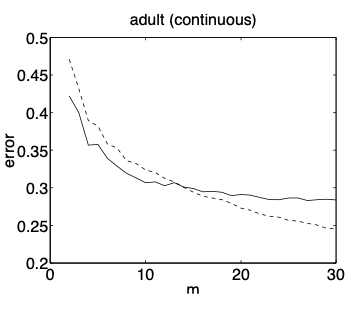
\includegraphics[scale=0.5]{figures/gen-disc}};
    		\node[fill=white,inner sep=1pt] (t1) at (2.5,3) {faster convergence};
         \draw[ultra thick,red,->] (t1) -- (7,2.5);
         \node[fill=white,inner sep=1pt] (t2) at (13,4.5) {higher asymptotic error};
         \draw[ultra thick,red,->] (t2) -- (10.5,2);
\end{tikzpicture}

Solid line: naive Bayes; dashed line: logistic regression.

\end{frame}

\end{document}
